\chapter{Metodología: herramientas y datos}\label{cap3}

En este capítulo se detallan las distintas herramientas y elementos utilizados en el trabajo. En primer lugar, se comienza por las librerías de Python utilizadas, continuando con los datos de estudio y los de apoyo y, terminando por los modelos de predicción.

\section{Liberías de Python}

Python \cite{python} es un lenguaje de programación interpretado de alto nivel que cuenta con multitud de librerías útiles para el análisis y la ciencia de datos. En este proyecto, las librerías utilizadas son:

\begin{itemize}
	\item Pandas.
	\item Scikit-learn.
	\item Matplotlib.
	\item Darts.
\end{itemize}

Pandas \cite{pandas} es una libería que permite el uso de \textit{dataframes}, unas estructuras de datos tabulares basada en columnas e índices, que facilitan realizar multitud de operaciones. Scikit-learn \cite{scikit-learn} es una librería de aprendizaje automático muy completa, de la que, en este trabajo, se utilizan sus herramientas para el cálculo de métricas de errores y el escalador de datos \textit{MinMaxScaler}. Matplotlib \cite{matplotlib}, por otra parte, es la libería base para la creación de gráficas en Python.

Darts \cite{darts} merece una mención especial, ya que es la base del proyecto. Se trata de una librería \textit{open-source} creada por la empresa suiza Unit8. Está especializada en la realización de predicciones en series temporales o \textit{forecasting}. Cuenta con multitud de modelos integrados, desde probabilísticos como ARIMA hasta modelos de \textit{deep learning} basados en PyTorch \cite{pytorch}, la plataforma que da soporte para la construcción y entrenamiento de los modelos. Simplifica el uso de distintos modelos utilizando un esquema común para entrenamiento y predicción, permitiendo realizar experimentos con múltiples modelos con facilidad. Cuenta además con herramientas tanto para el preprocesamiento de los datos como para el análisis posterior.

\section{Series de datos de estudio}

En la empresa de recambios de automóvil de estudio, las distintas referencias se agrupan en familias de productos para recibir un tratamiento común independientemente de la marca. Por ejemplo, dentro de las baterías existen distintas marcas de proveedores con diferentes características, por lo que reciben una referencia única. Todas estas referencias se agrupan dentro de una familia, denominada baterías, que engloba el conjunto de referencias de productos con características generales similares pero especificaciones técnicas diferentes que satisfacen un mismo mercado y una misma demanda. 

Los datos que se obtienen del ERP son el agrupado de ventas diarias de cada familia de estudio. Las familias de producto utilizadas en este estudio son las siguientes:

\begin{itemize}
    \item Baterías.
    \item Filtros.
    \item Aceites.
    \item Limpiaparabrisas.
\end{itemize} 

Relativo al rango de fechas de los datos extraídos se incluyen desde el inicio de la empresa a mediados de 2008 hasta la mitad del año 2024. Con el fin de evitar desviaciones externas a las variables que se incluyen en el estudio, se escogen los datos desde el 1 de enero de 2012 hasta el 31 de diciembre de 2023 evitando el periodo de comienzo de actividad empresarial. De la muestra se excluyen los datos del primer semestre del año 2024 como método de testeo y validación de los modelos predictivos objeto de entreno y estudio en este proyecto. Adicionalmente, la extracción de datos se ha ajustado al periodo de actividad de la tienda, que es de lunes a viernes, excluyendo los fines de semana para facilitar el trabajo de los modelos matemáticos. Sin embargo, para mantener coherencia en el conjunto de datos, se incluyen los días festivos que sea entre semana, que tendrán 0 unidades vendidas.

Los datos se encuentran en un archivo .csv y se cargan en Python en un \textit{DataFrame} de la librería Pandas \cite{pandas}. A continuación, en la Tabla \ref*{3-cabezafiltros} se observa una muestra con los cinco primeros datos como referencia de la estructura de los datos de las series.

\begin{table}[H]
	\ttabbox[\FBwidth]
	{\caption{Cabeza de la serie histórica de ventas de filtros}\label{3-cabezafiltros}}
	{\begin{tabular}{|c|c|}
		\hline
        \textbf{Fecha} & \textbf{Unidades vendidas} \\
        \hline
        2010-01-01 & 0 \\
        \hline
        2010-01-04 & 4 \\
        \hline
        2010-01-05 & 3 \\
        \hline
        2010-01-06 & 0 \\
        \hline
        2010-01-07 & 10 \\
        \hline
	\end{tabular}}
\end{table}


\subsection{Baterías}

Las baterías forman un grupo de producto que resulta relevante de estudio, debido a que son un elemento común a todos los vehículos que puede considerarse consumible, ya que con el tiempo se degradan y es necesaria su sustitución. Además, son un elemento perecedero y por ello es necesario que pasen en el almacén el menor tiempo posible para evitar posibles fallos y, posteriores devoluciones por garatía. También hay que tener en cuenta que las baterías son productos más voluminosos y pesados que el resto de productos, por lo que el coste de inventario es superior a la media de los demás productos.

En la Figura \ref*{3-graf_baterias}, se observa una gráfica de la serie temporal, donde se muestra una clara tendencia al alza y cierta estacionalidad. Además, a destacar el bajón de ventas producidas por el confinamiento durante el COVID y el posterior incremento de las ventas al ser diferidas.

\begin{figure}[H]
	\ffigbox[\FBwidth] {
	\caption{Gráfica de la serie temporal de ventas de baterías}\label{3-graf_baterias}
	}
	{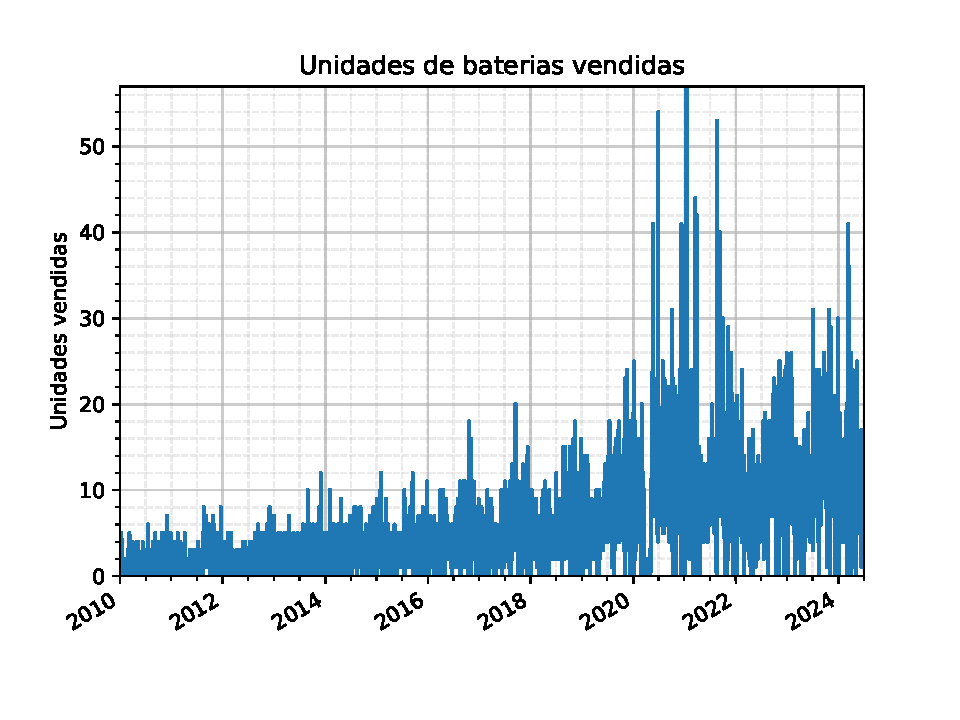
\includegraphics[width=0.75\textwidth]{imagenes/grafica_baterias.pdf}}
\end{figure}

Utilizando la librería Prophet \cite{prophet}, se desglosa la estacionalidad de la serie temporal, mostrada en la Figura \ref*{3-comp_baterias}. La primera subgráfica muestra la tendencia al alza en las ventas de esta familia. La segunda, muestra la estacionalidad intrasemanal, donde muestra que la mayoría de ventas se producen a comienzo de semana. En la última, la estacionalidad anual muestra que las ventas entorno al mes de abril son las más bajas del año, mientras que a partir de septiembre se incrementan considerablemente.

\begin{figure}[H]
	\ffigbox[\FBwidth] {
	\caption{Gráfica de componentes de la serie de baterías}\label{3-comp_baterias}
	}
	{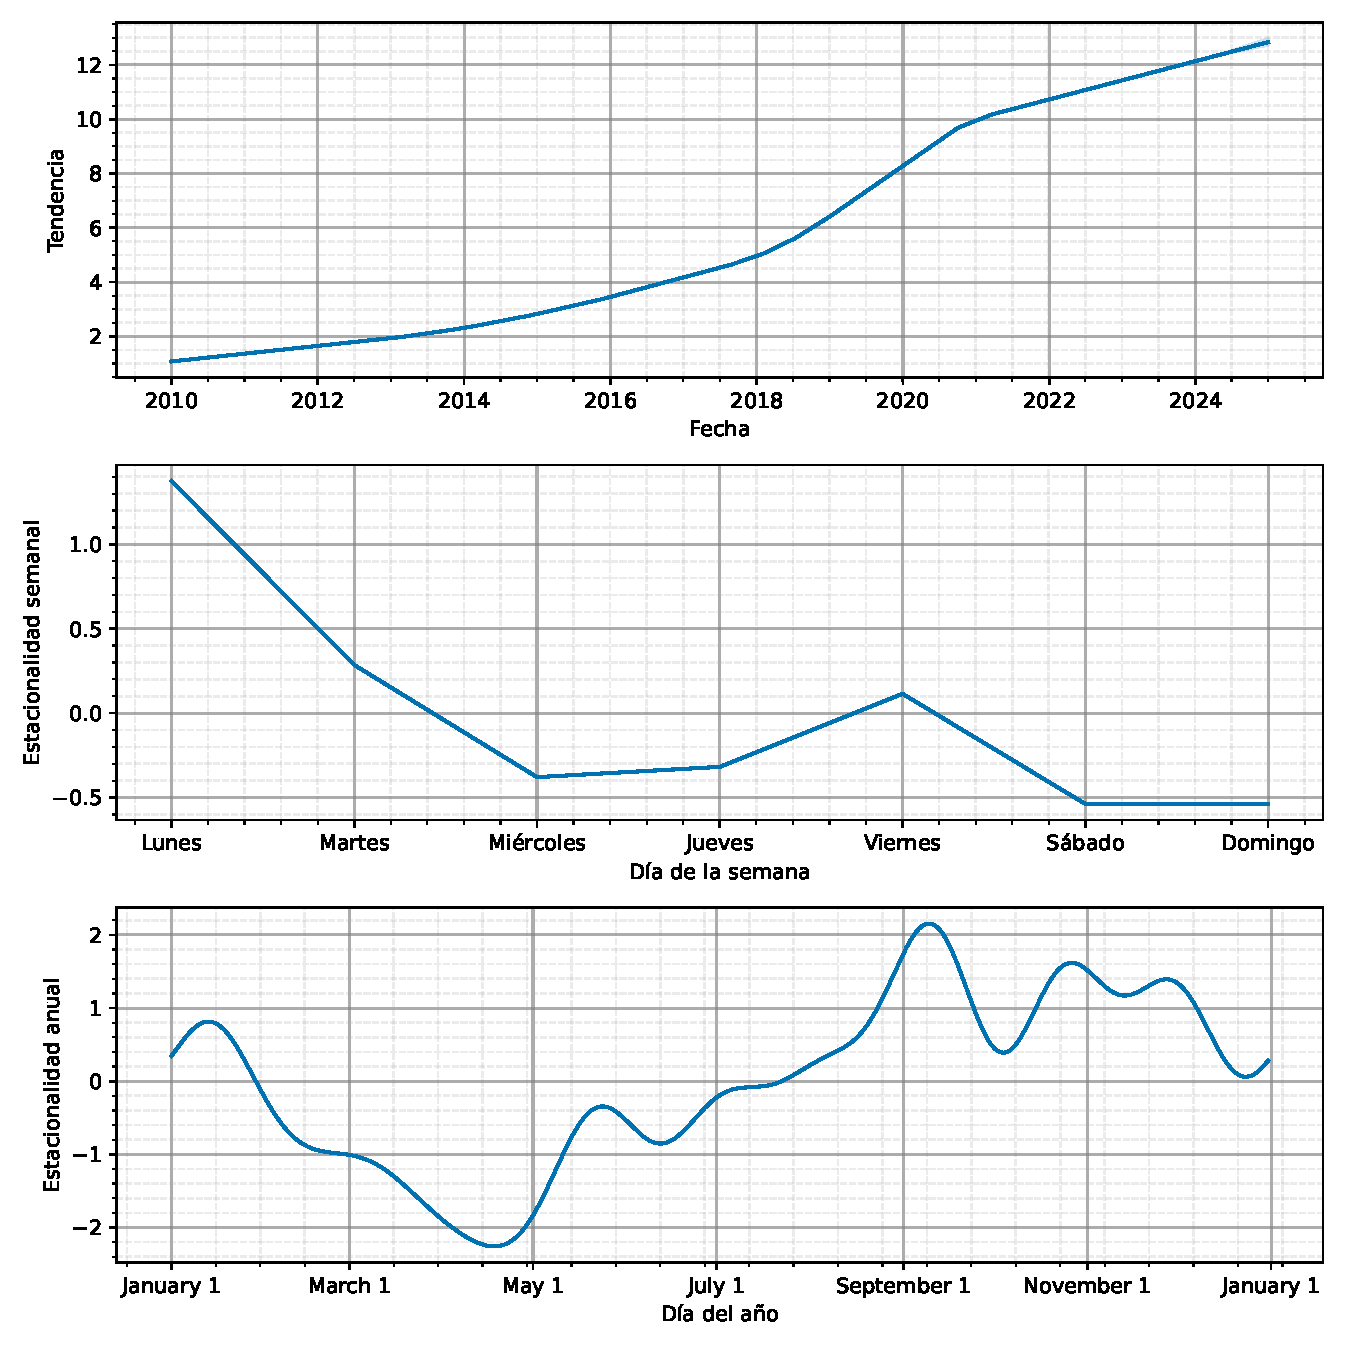
\includegraphics[width=0.75\textwidth]{imagenes/comps_baterias.pdf}}
\end{figure}


\subsection{Filtros}

Los filtros son el consumible por excelencia de los vehículos con motores de combustión, ya que la sustitución periódica de filtros como el de aceite y el de combustible es esencial para alargar la vida útil del motor. Además, ciertos filtros, como el del aire, están presentes en todo tipo de vehículos, ya sean clásicos de combustión o bien más modernos como híbridos o eléctricos, por lo que se conforma una familia de producto que tiene un alto volumen de ventas.

En la Figura \ref*{3-graf_filtros} se observa el histórico de datos de la familia de filtros. No se aprecia tanta estacionalidad como en el caso de las baterías, pero la tendencia al alza es bastante clara en los primeros años, con un estancamiento a partir del año 2020.

\begin{figure}[H]
	\ffigbox[\FBwidth] {
	\caption{Gráfica de la serie temporal de ventas de filtros}\label{3-graf_filtros}
	}
	{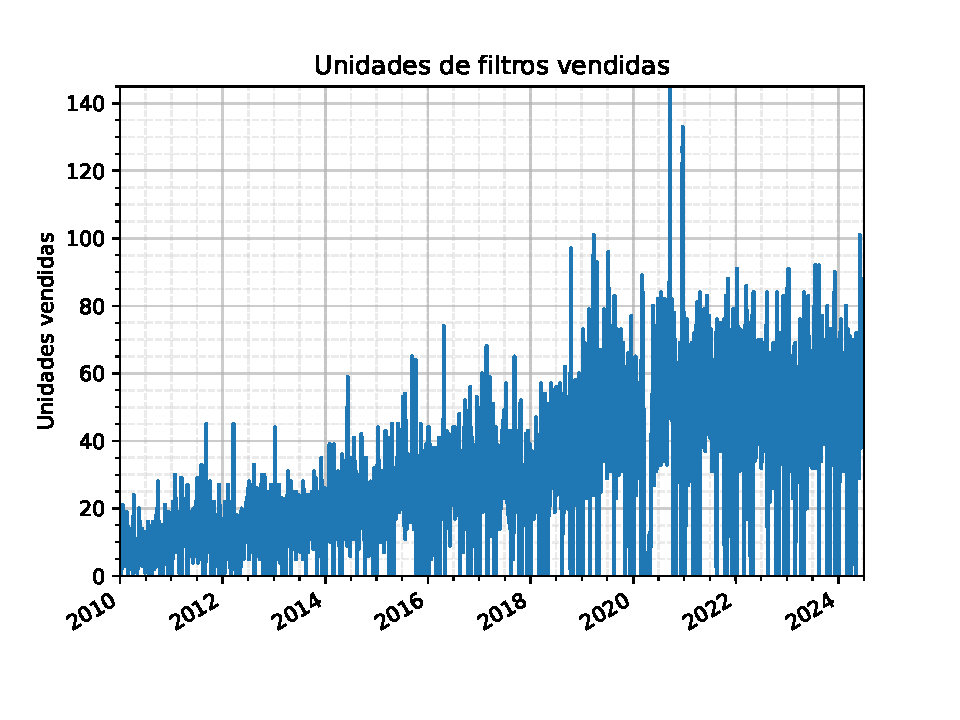
\includegraphics[width=0.75\textwidth]{imagenes/grafica_filtros.pdf}}
\end{figure}

Desglosando los componentes estacionales, no se observa una estacionalidad muy marcada a nivel semanal, pero sí a nivel anual, donde la mayoría de mantenimientos se realizan previos a períodos vacacionales.

\begin{figure}[H]
	\ffigbox[\FBwidth] {
	\caption{Gráfica de componentes de la serie de filtros}\label{3-comp_filtros}
	}
	{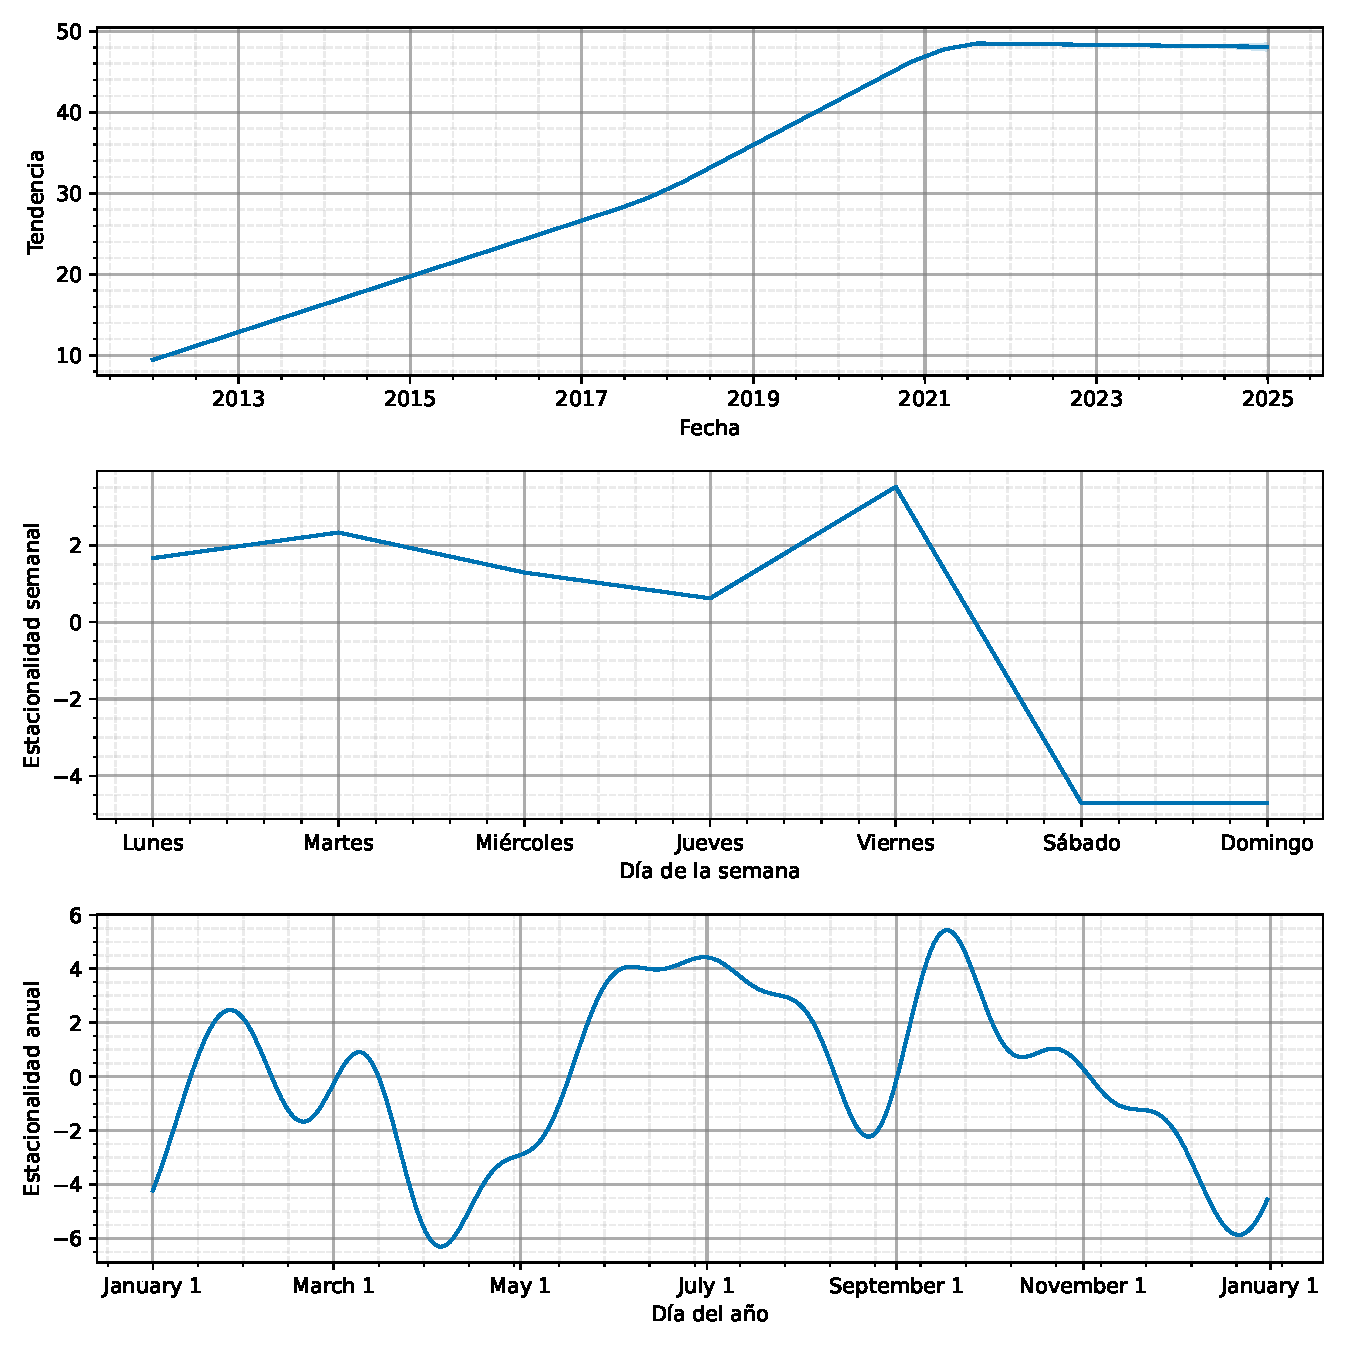
\includegraphics[width=0.75\textwidth]{imagenes/comps_filtros.pdf}}
\end{figure}

\subsection{Aceites}

Otra familia importante es la de los aceites industriales. Se trata de productos que suelen ser voluminosos y, al igual que los filtros, su sustitución es imprescindible para un correcto funcionamiento de los vehículos ya que de ello depende la correcta lubricación de las partes del motor y elementos móviles y, por lo tanto, alargar su vida útil. En la Figura \ref*{3-graf_aceites} se muestra la gráfica de la serie histórica.

\begin{figure}[H]
	\ffigbox[\FBwidth] {
	\caption{Gráfica de la serie temporal de ventas de aceites}\label{3-graf_aceites}
	}
	{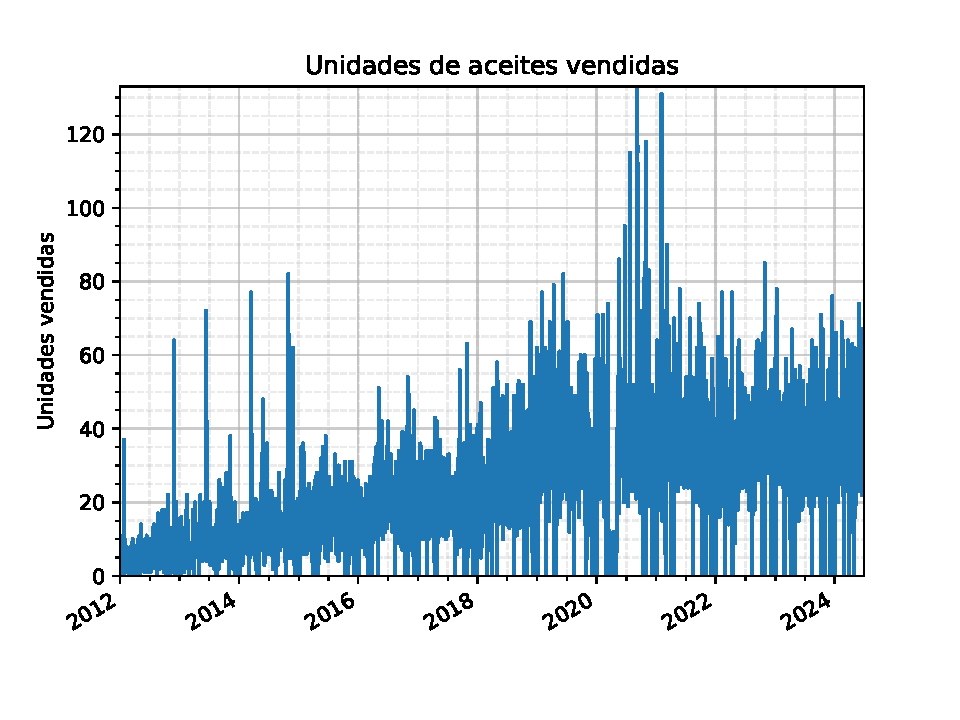
\includegraphics[width=0.75\textwidth]{imagenes/grafica_aceites.pdf}}
\end{figure}

En la Figura \ref*{3-comp_aceites} se muestra el desglose de los componentes de la serie. A nivel semanal es de resaltar que los viernes hay un mayor número de ventas, mientras que a nivel anual se observa que la estacionalidad es trimestral. Se nota un incremento de la demanda desde 2012 hasta 2020, donde, aislando la repercusión del efecto COVID que desvía la tendencia, parece estancarse desde el 2020 hasta el 2024

\begin{figure}[H]
	\ffigbox[\FBwidth] {
	\caption{Gráfica de componentes de la serie de aceites}\label{3-comp_aceites}
	}
	{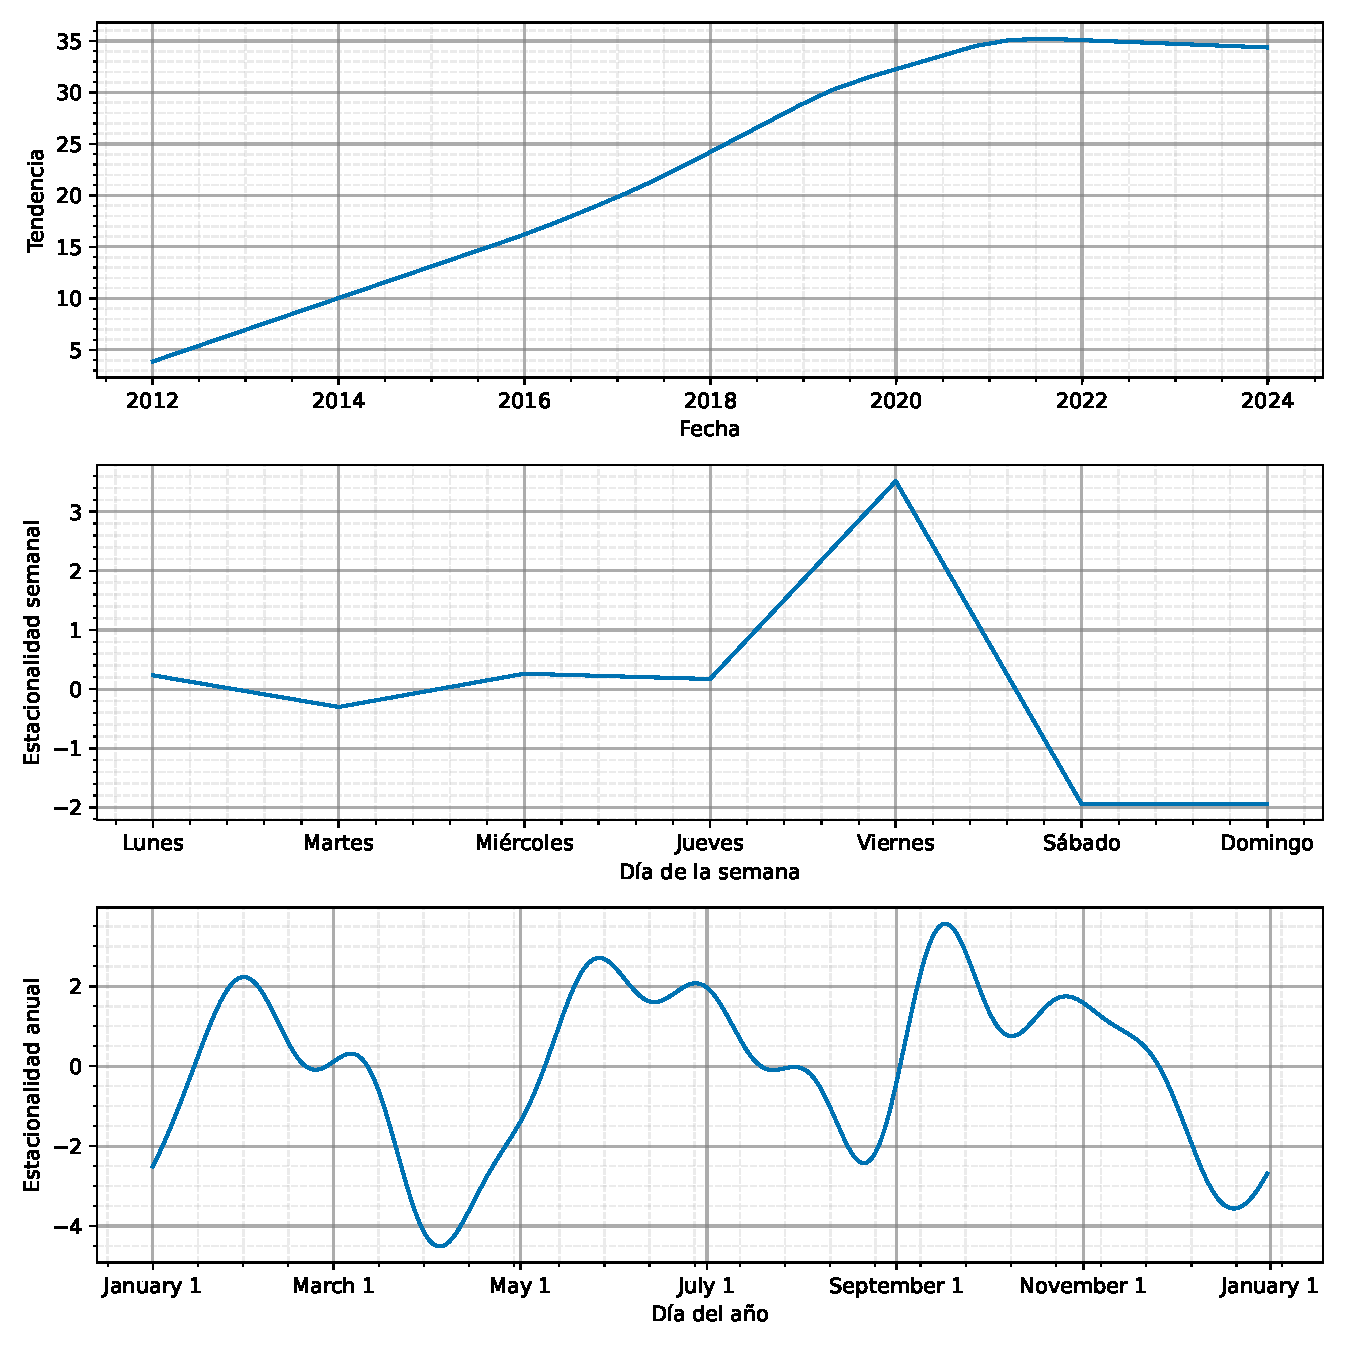
\includegraphics[width=0.75\textwidth]{imagenes/comps_aceites.pdf}}
\end{figure}

\subsection{Limpiaparabrisas}

Los limpiaparabrisas son un tipo de producto con una clara estacionalidad, ya que durante la época con mayor irradiación solar se deterioran en coches estacionados en la calle y se sustituyen cuando empieza la época de lluvias y es fundamental para la correcta visibilidad de los vehículos. En la Figura \ref*{3-graf_limpiaparabrisas}, se observa como hay picos intensos de demanda y valles marcados.

\begin{figure}[H]
	\ffigbox[\FBwidth] {
	\caption{Gráfica de la serie temporal de ventas de limpiaparabrisas}\label{3-graf_limpiaparabrisas}
	}
	{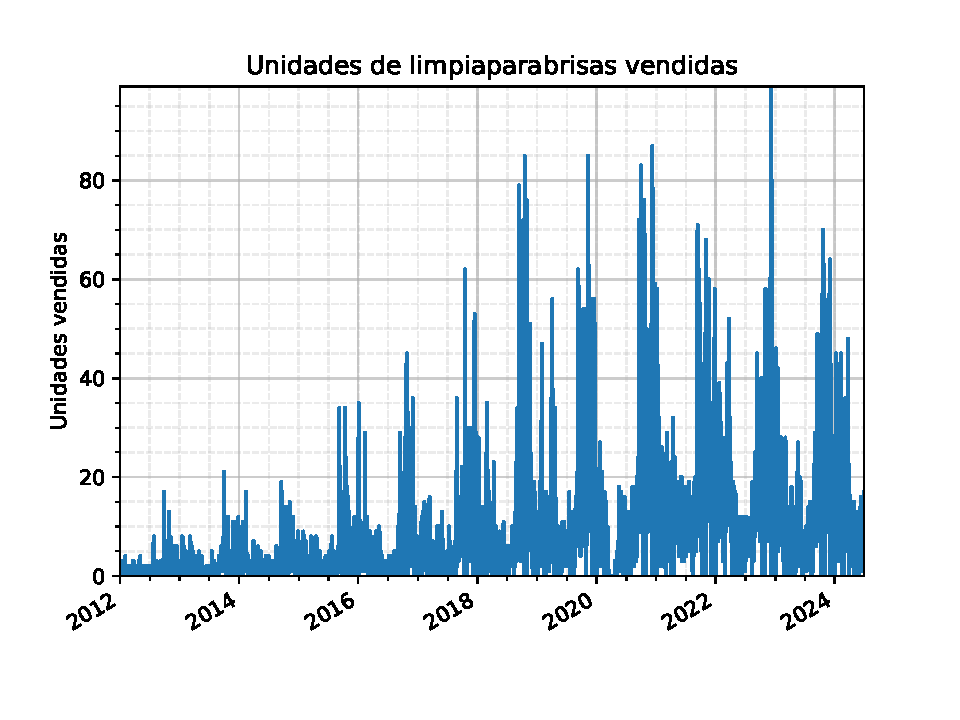
\includegraphics[width=0.75\textwidth]{imagenes/grafica_limpiaparabrisas.pdf}}
\end{figure}

En la Figura \ref*{3-comp_limpiaparabrisas} se observan el incremento de las ventas a lo largo de la serie histórica y la estacionalidad que concentra las ventas después de la época de verano.

\begin{figure}[H]
	\ffigbox[\FBwidth] {
	\caption{Gráfica de componentes de la serie de limpiaparabrisas}\label{3-comp_limpiaparabrisas}
	}
	{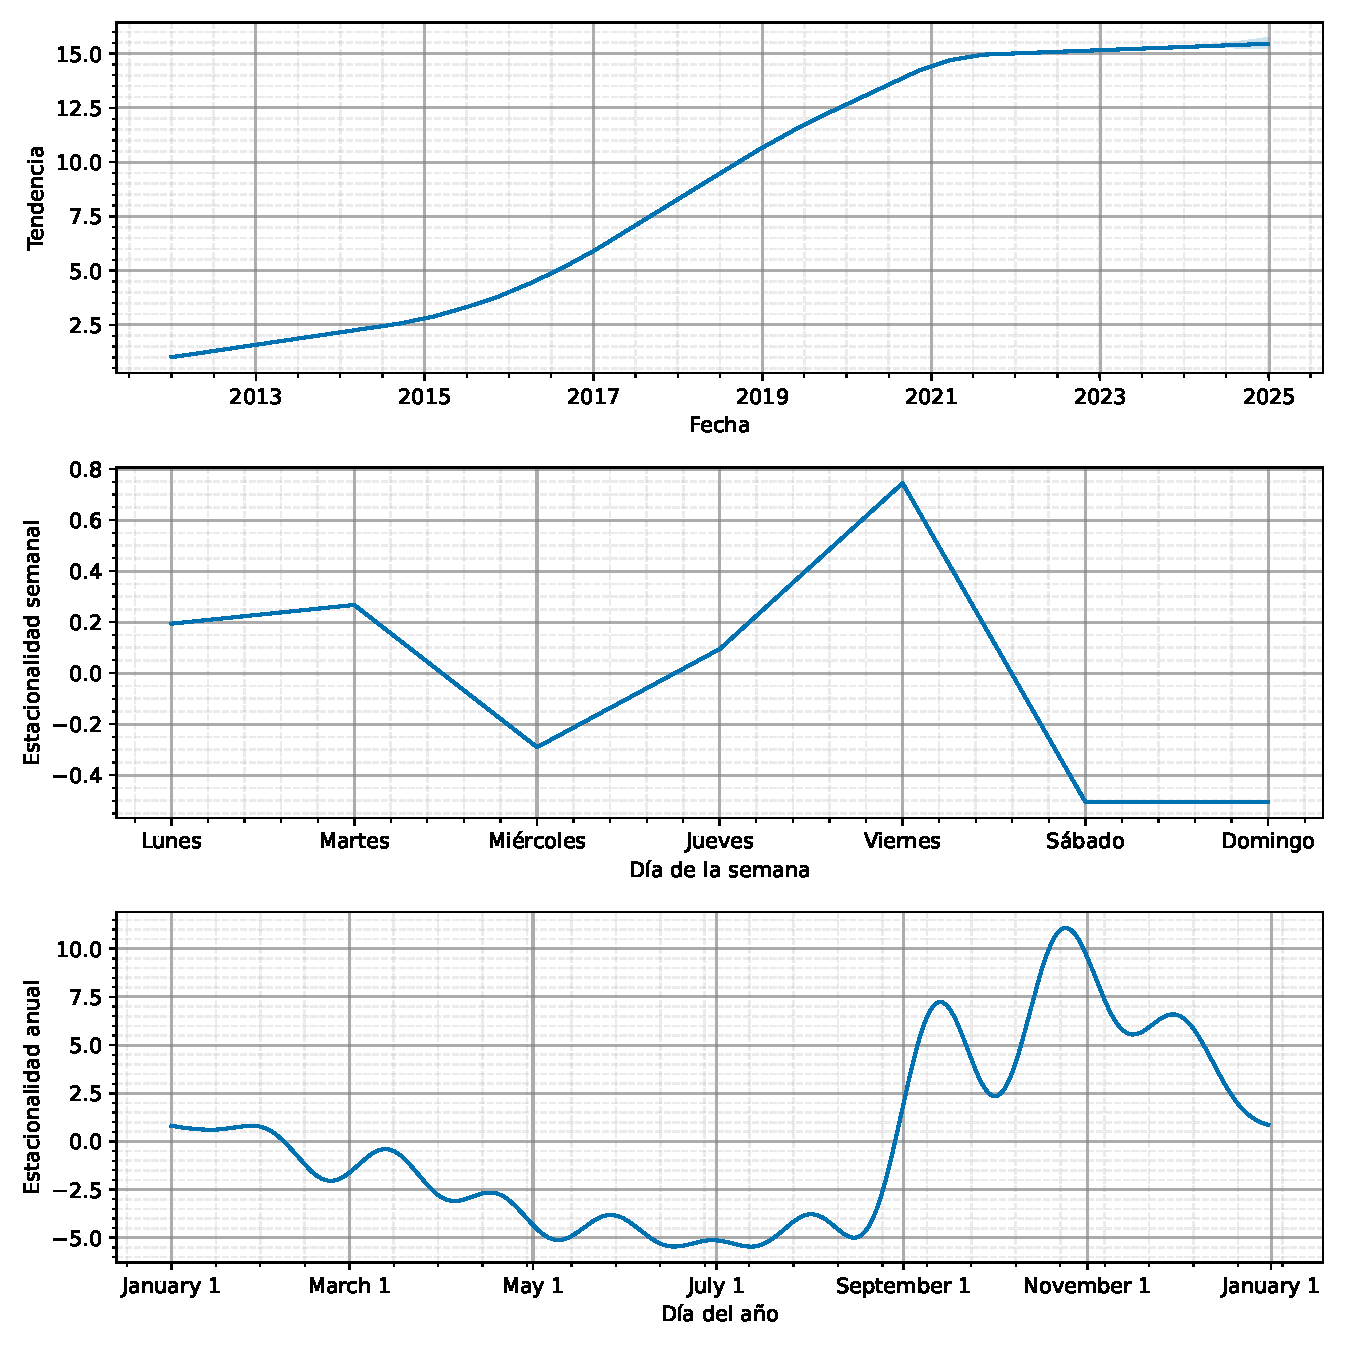
\includegraphics[width=0.75\textwidth]{imagenes/comps_limpiaparabrisas.pdf}}
\end{figure}


\section{Regresores externos}

A pesar de que el enfoque de las predicciones es univariable, ya que solo se busca predecir el valor de las ventas, es posible añadir regresores externos o \textit{covariates} para mejorar la calidad de los resultados. Estos regresores pueden ser pasados, futuros o estáticos. En función del modelo, admiten de un tipo u otro.

\subsection{Días festivos}

Los días festivos las tiendas permanecen cerradas, por lo que las ventas son cero. Como las series de datos de estudio recogen todos los días de lunes a viernes incluyendo los festivos, es buena idea añadir como regresor una serie donde se indique los días que son festivos. En este sentido, la librería Darts añade la funcionalidad de añadir una serie extra con los días laborables de España y, además, de Andalucía. Se trata de una serie con una variable binaria donde 1 indica que es día festivo y 0 indica que no lo es. Se puede observar en la Figura \ref*{3-dias_festivos} los días festivos durante el rango de fechas del caso de estudio.

Además, algunos modelos utilizados cuentan con la posiblidad de utilizar \textit{covariates} futuras. Por ello, los que lo permitan, utilizarán los datos de los días festivos para realizar las predicciones en el periodo de predicción.

\begin{figure}[H]
	\ffigbox[\FBwidth] {
	\caption{Días festivos de España y Andalucía}\label{3-dias_festivos}
	}
	{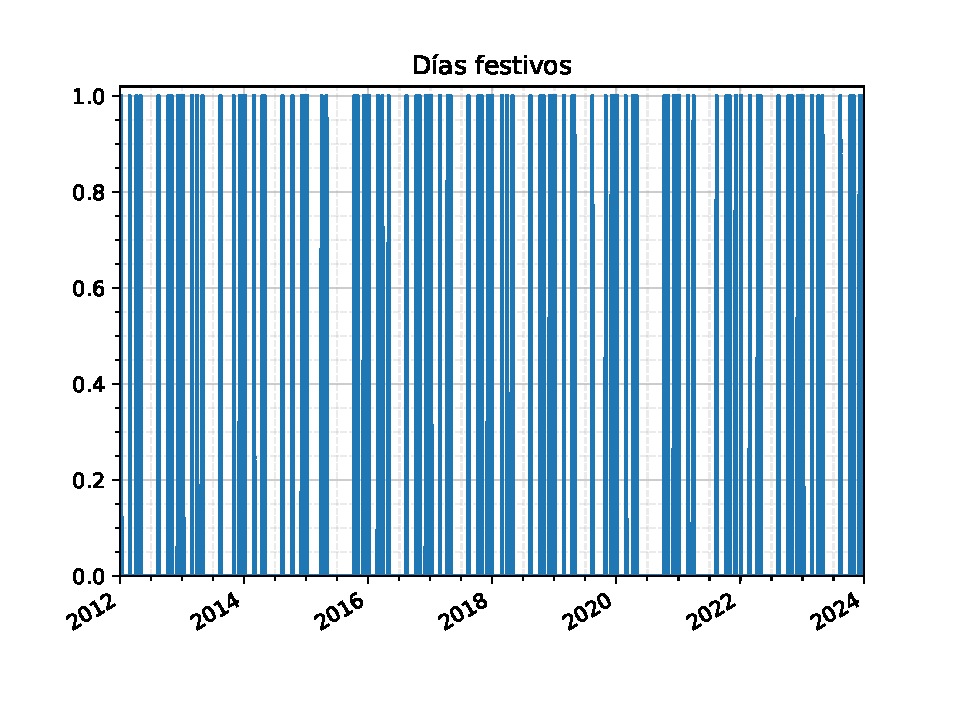
\includegraphics[width=0.75\textwidth]{imagenes/grafica_holidays.pdf}}
\end{figure}

\subsection{Meteorología}

Las precipitaciones y la temperatura son elementos que causan desgaste en los vehículos. Además, estas variables son estacionales, por lo que puede favorecer la comprensión de comportamientos de las series de datos por parte de los modelos.

Para ello, se toman datos provistos por Agencia Estatal de Meteorología en la plataforma AEMET OpenData \cite{aemet}. Los datos obtenidos pertenecen a las climatologías diarias recogidas en la estación meteorológica de Olvera, en la provincia de Cádiz. Esta localidad se encuentra localizada aproximadamente en el centro geográfico de todas las tiendas de la empresa y tras realizar un muestreo aleatorio se puede concluir que su climatología es extrapolable al resto.

De todos los datos que ofrece la plataforma, se toman la temperatura media diaria, las precipitaciones y la humedad media diaria. En la Figura \ref*{3-meteo} se muestra una gráfica de los datos en el rango temporal del estudio. Se observa la estacionalidad de los datos de temperatura y humedad, ya que son variables con poca dispersión diaria. Por otro lado, las precipitaciones son datos puntuales, aunque suelen aparecer en las mismas fechas de cada año.

\begin{figure}[H]
	\ffigbox[\FBwidth] {
	\caption{Gráfica de los datos meteorológicos}\label{3-meteo}
	}
	{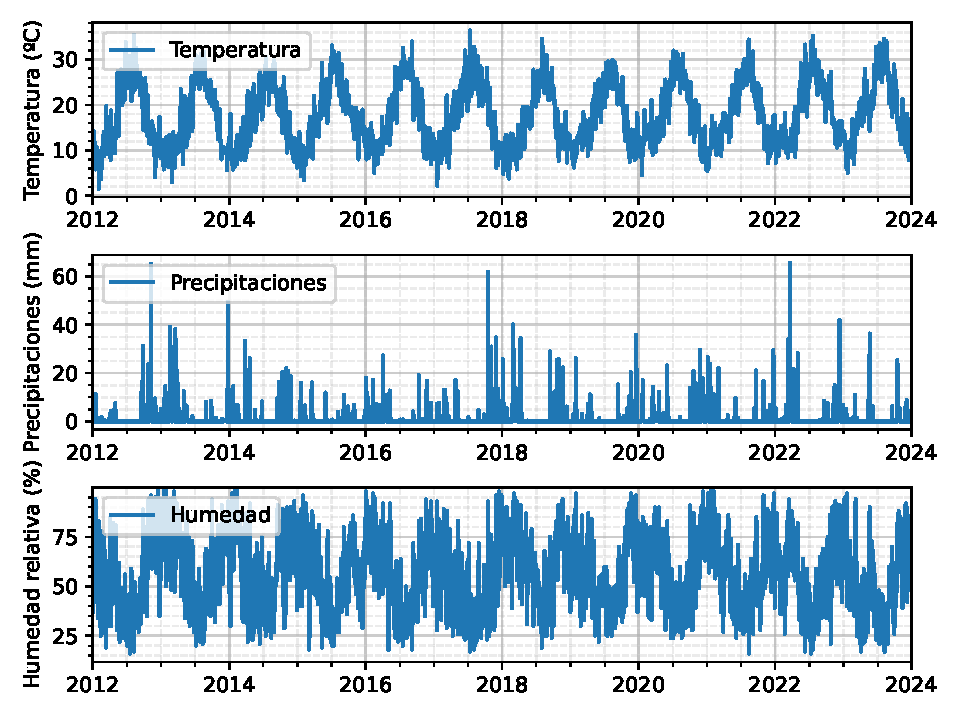
\includegraphics[width=0.75\textwidth]{imagenes/grafica_meteo.pdf}}
\end{figure}


\subsection{Precio del carburante}

El precio de los combustibles fósiles influye en la industria de la automoción en gran medidsa, ya que su valor incrementa el coste de la movilidad en vehículos térmicos. Por ello, su precio puede influir en la industria del \textit{aftermarket} del automóvil al verse reducido el uso de los vehículos. Por ello, al verse reducido el uso de los vehículos, así que es interesante utilizar esta variable como regresor.

Se utilizan datos obtenidos del Boletín del Petróleo de la Comisión Europea \cite{petrol} que provee datos semanales del precio de diversos combustibles en todos los países de la Unión Europea. Como el diésel y la gasolina son los carburantes más empleados en la mayoría de vehículos serán los empleados en el estudio. Los datos obtenidos son semanales mientras que nuestros datos son diarios, por lo que el valor de cada semana se extenderá a todos los días de esa semana. 

La Figura \ref*{3-precio_combustible} muestra la evolución del precio de ambos combustibles a lo largo del período del estudio.

\begin{figure}[H]
	\ffigbox[\FBwidth] {
	\caption{Evolución del precio del combustible en España}\label{3-precio_combustible}
	}
	{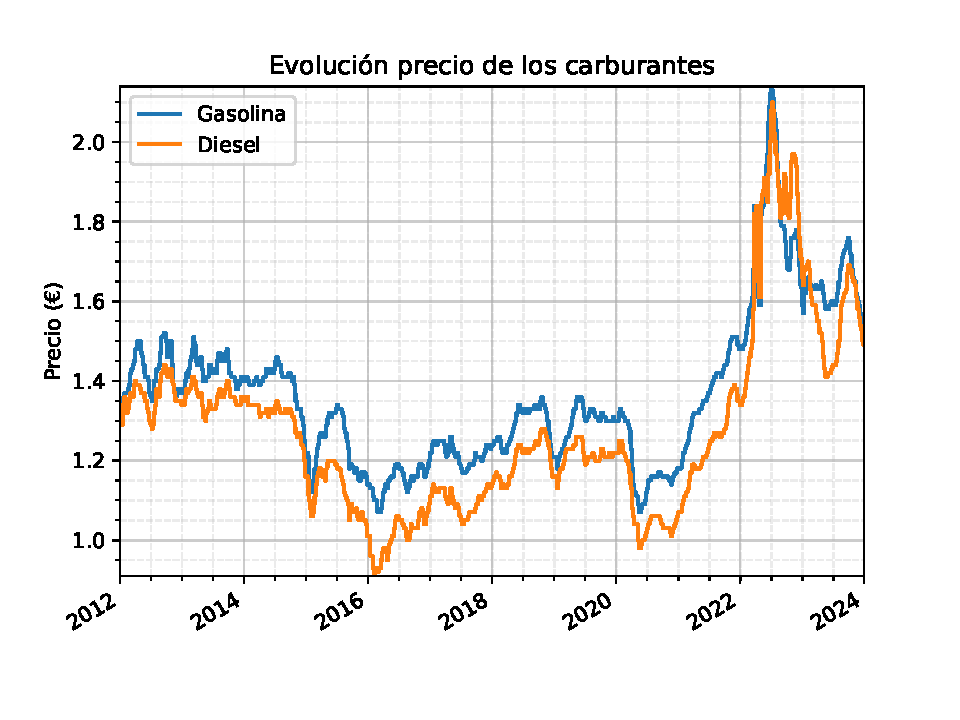
\includegraphics[width=0.75\textwidth]{imagenes/grafica_carburantes.pdf}}
\end{figure}

\subsection{Regresores cíclicos temporales}

Los datos de estudio del proyecto cuentan con cierta estacionalidad, por ello, los datos de ventas se ven influenciados por el momento en el que se produce. Por lo tanto, es útil añadir series temporales que indiquen el momento de los distintos períodos del año.

Darts integra la posibilidad de generar ciertos patrones que se repiten de forma cíclica durante el tiempo y añadir más factores tanto para el entrenamiento como para las previsiones. Estos patrones temporales y añaden variables adicionales que en función de la fecha cuentan con diferentes valores. Los patrones añadidos son los siguientes:

\begin{itemize}
	\item Día de la semana.
	\item Día del mes.
	\item Día del año.
	\item Mes del año.
	\item Cuatrimestre del año. 
\end{itemize}

Cuando se utilizan patrones cíclicos para entrenar modelos de inteligencia artificial se suele aplicar trigonometría \cite{sincos} a estas variables. Esto permite a los modelos capturar de forma óptima el comportamiento cíclico. Por ello, cada variable se añaden como pares, siendo una el seno y otra el coseno de la variable.

Como estos patrones se pueden replicar para todos los rangos temporales, los modelos que utilicen regresores futuros podrán utilizarlos para mejorar sus predicciones.